\section{Introduction}

\begin{figure*}[t]
    \vspace{-10pt}
    \centering
    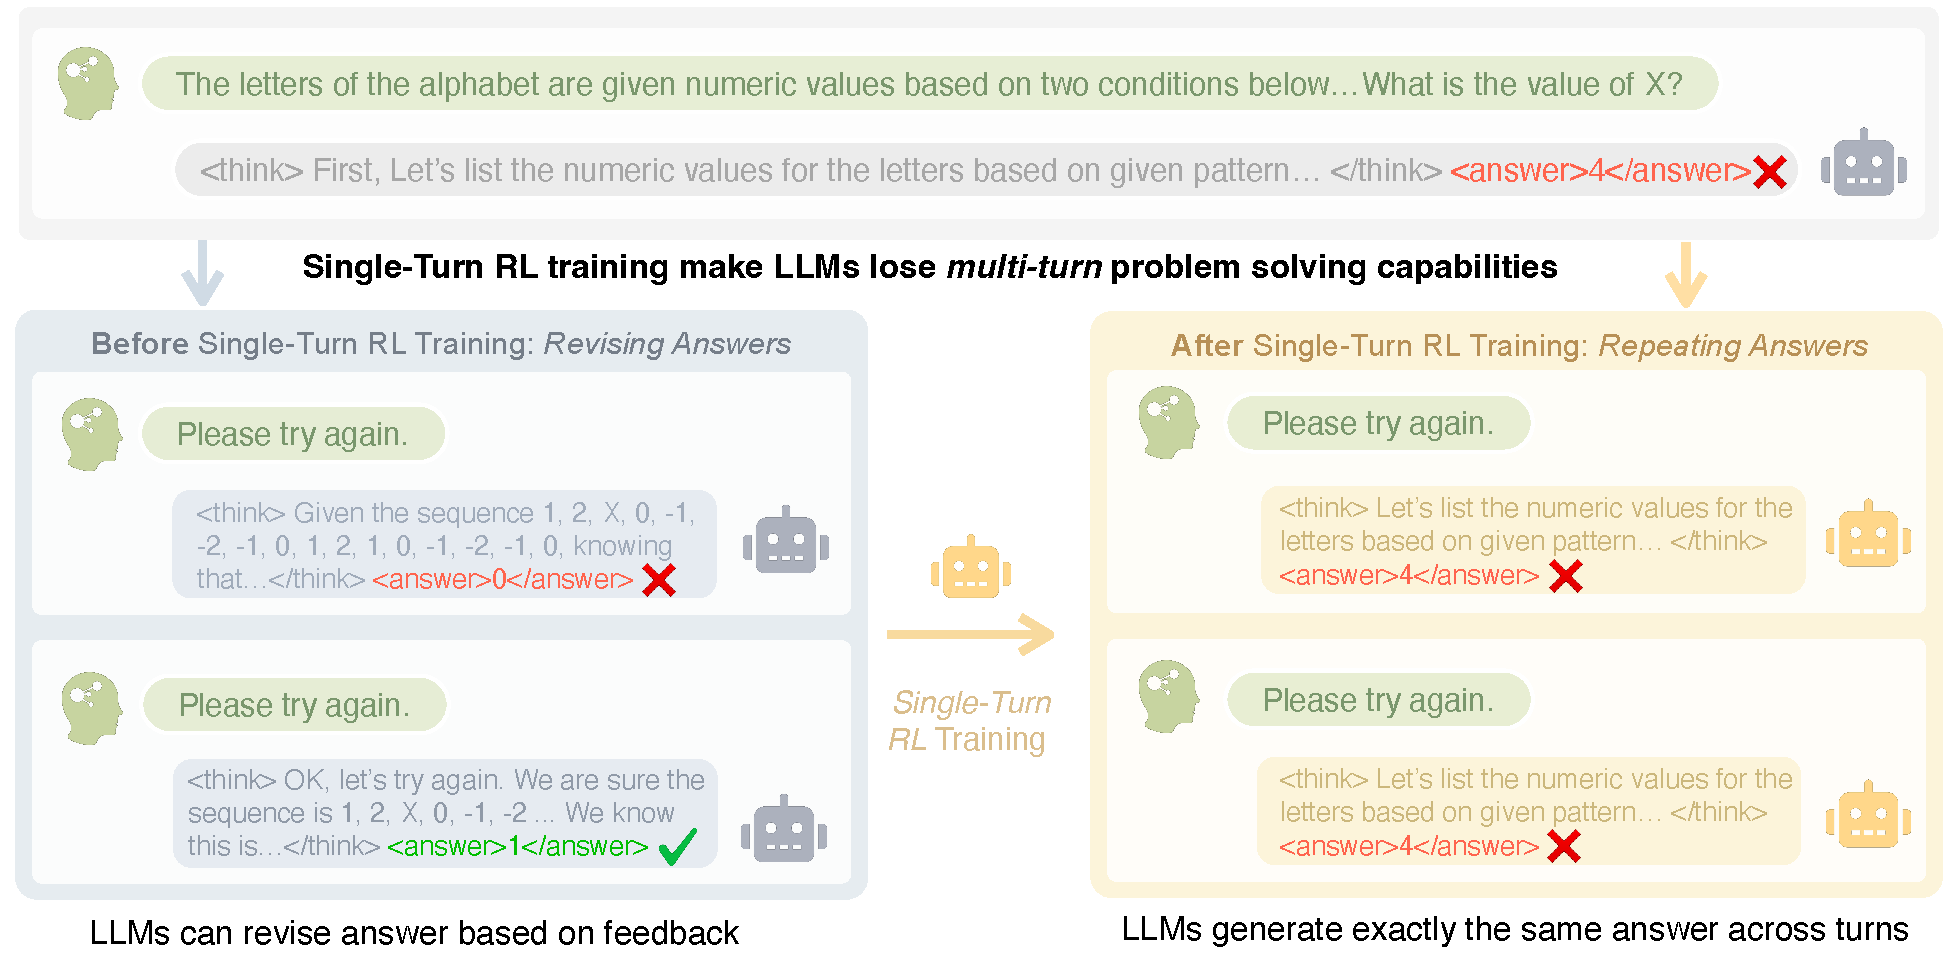
\includegraphics[width=\textwidth]{figures/fig2.pdf}
    \vspace{5pt}
    \caption{Single-turn RL causes LLMs to repeat the same answer across turns instead of revising based on feedback.}
    \label{fig:example}
\end{figure*}

Large language and reasoning models (LLMs/LRMs)~\citep{deepseekr1, gpt4, qwen25, gemini} have demonstrated strong capabilities in solving complex tasks such as mathematics problems and code generation. Recent advances in reinforcement learning (RL)~\citep{deepseekr1, ppo, archer, ragen} further enhance the reasoning capabilities of LLMs through verifiable reward frameworks (RLVR). However, many real-world applications like chatbots, programming assistants, and educational tools~\citep{osworld, swegym, webshop, alfworld, mint} require models to engage in multi-turn problem solving and adapting their reasoning with feedback. Despite this need, it remains underexplored how models trained with single-turn RL can generalize to interactive, multi-turn problem-solving.

In this work, we first observe that single-turn RL can hinder a model’s ability to engage in interactive multi-turn reasoning. Specifically, single-turn-trained models often fail to incorporate in-context feedback and instead \textbf{persist with their initial answers across subsequent turns} (Figure~\ref{fig:example}). To quantify this persistence, we define \textit{effective answer} as a new response that has never been explored in any previous turn by the LLM. In Figure~\ref{fig:answer_repetition}, we observed that in 70\% of the failed cases, the single-turn-trained models generate exactly the same answer across five turns (i.e. only 1 effective answer). One particular reason for that is that most existing datasets are inherently single-turn and lack signals for iterative exploration. Without such signals, models have limited opportunities to explore diverse reasoning paths or adapt their strategies based on feedback. This challenge motivates our research question: \textit{How can we train language models to iteratively explore and refine their reasoning, especially when initial attempts fail and only minimal feedback is available?}

\begin{wrapfigure}{r}{0.42\textwidth}
% \begin{figure}[t]
    \vspace{-12pt}
    \centering
    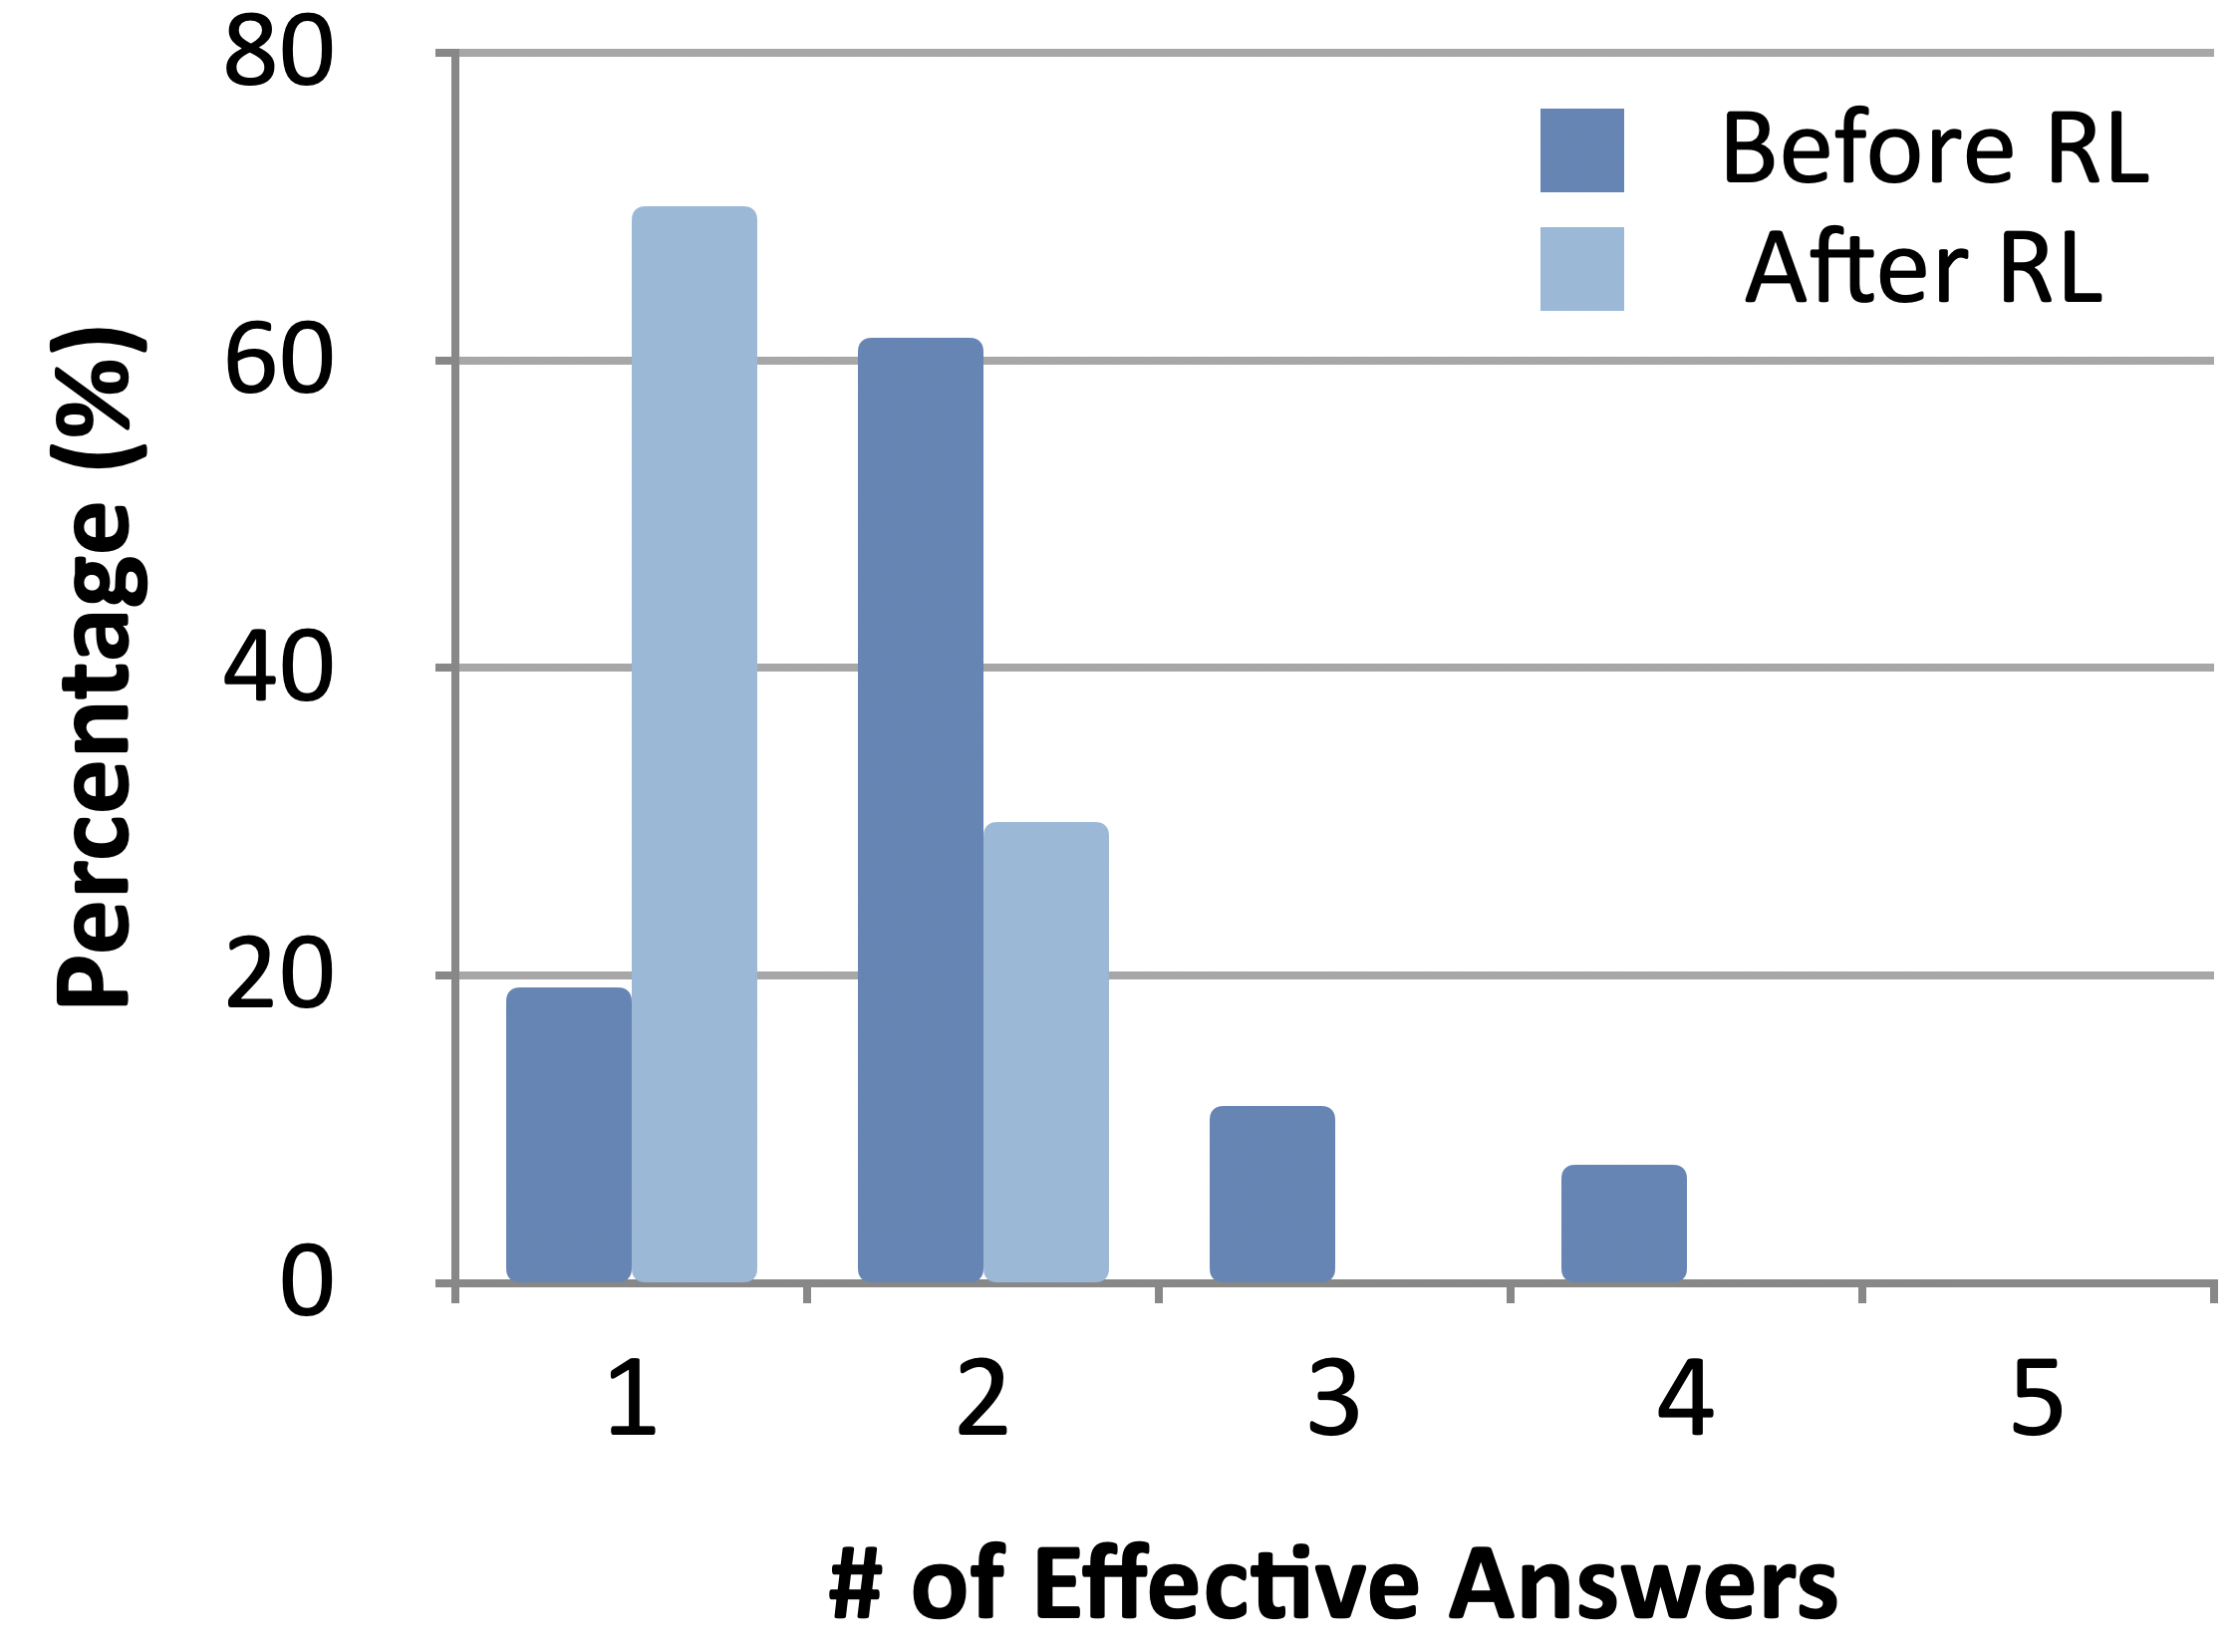
\includegraphics[width=\linewidth]{figures/validation_comparison.png}
    \vspace{-5pt}
    \caption{After single-turn RL training, the model gives exactly the same answer across five interaction turns in 70\% of the cases.}
    \label{fig:answer_repetition}
    % \vspace{-10pt}
% \end{figure}
\end{wrapfigure}

Collecting real-world multi-turn user feedback, however, is expensive and logistically difficult. Constrained by this data bottleneck, the existing multi-turn framework has been training in automatic feedback such as code interpreter messages~\citep{osworld, swegym, mint} and embodied simulator signals~\citep{alfworld, simworld}. Although useful, these signals are costly to construct and are still limited in scope~\citep{cao2025skyrl}. In light of these limitations, we explore a simple yet effective framework that can leverage static dataset for multi-turn RL training. By inserting minimal verbal feedback ("try again") into the context, we encourage models to revise and explore alternative reasoning paths. We call this \textbf{Unary Feedback as Observation} (UFO), framing interactive problem-solving as Markov Decision Processes (MDP) where the model only receives unary feedback as its environmental observation.

Through experiments, we show that applying UFO in multi-turn RL effectively encourages interactive reasoning and helps the model explore alternative reasoning paths across turns. Instead of repeating previous answers, UFO trained models adjust their problem-solving strategies based on prior outcomes, leading to a 14\% improvement in multi-turn success rates over conventional single-turn RL. Furthermore, we find that the model’s ability to self-reflect and adapt its reasoning generalizes robustly across diverse out-of-domain tasks. 

To further align model behavior with real-world multi-turn reasoning objectives, we propose two guiding principles: \textbf{minimality}, where models should minimize the number of interaction turns needed to reach a correct answer, and \textbf{diversity}, where they should explore varied strategies when faced with failure. To operationalize these principles, we introduce a turn-wise reward decay and an answer repetition penalty which encourage systematic planning and improve reasoning efficiency.

To summarize, our contributions are as follows:
\begin{itemize}[leftmargin=*, itemsep=0em, topsep=0pt]
    \item We identify that while current single-turn RL training improves reasoning, they can lead to repetitive and degraded outputs in multi-turn, interactive reasoning scenarios.
    \item We explore a simple yet effective framework, \textbf{Unary Feedback as Observation (UFO)}, to enable multi-turn RL training on existing static single-turn reasoning datasets.
    \item We show that turn-wise reward decay and answer repetition penalty could effectively improve multi-turn reasoning minimality and diversity.
\end{itemize}


\begin{figure*}[t]
    \centering
    \vspace{-12pt}
    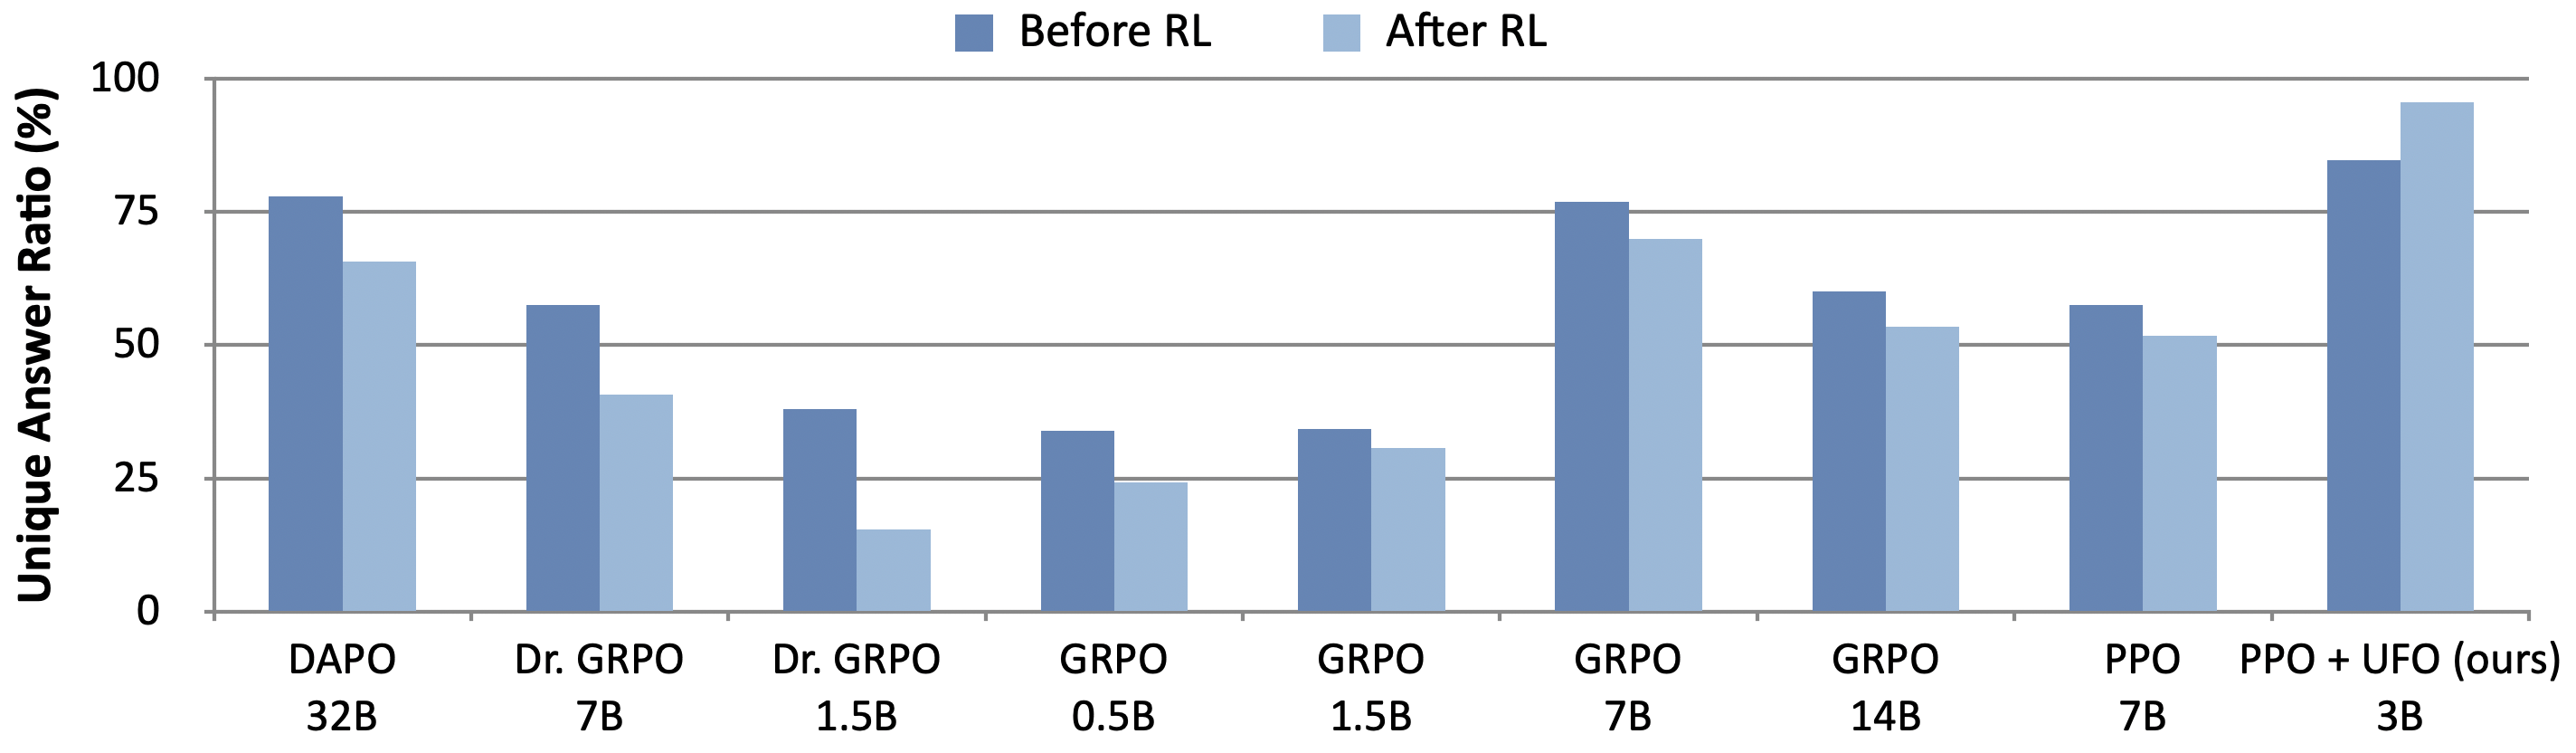
\includegraphics[width=0.98\linewidth]{figures/unique_aswer_ratio_comparison.png}
    \vspace{10pt}
    \caption{\textbf{Comparison of effective (unique) answer ratio (\%) before and after RL training}. Across single-turn RL methods, the unique answer ratio consistently drops after training across multiple model scales.}
    \vspace{5pt}
    \label{fig:compare_unique}
\end{figure*}
